


\begin{frame}{%
  \begin{minipage}[t]{0.85\textwidth}
    Brushane
  \end{minipage}%
  \hfill
  \begin{minipage}[t]{0.1\textwidth}
    \raggedleft
    
\includegraphics[width=0.55cm, height=0.55cm, keepaspectratio]{Billeder/Ikoner/star.png}%
  \end{minipage}%
} 
  \vspace{0.25em}
  \begin{columns}[T]
    % --- Venstre kolonne: Tekst ---
    \column{0.55\textwidth}
    \setlength{\parskip}{0.5em}
    \small
    \RaggedRight\textbf{\textit{Calidris pugnax}} – stor vadefugl som tilhører sneppefuglene \par

    \textbf{Udseende:} \\
    \quad – Kort svagt nedadbøjet næb. Giraf-hals. Uproportionelt lille hoved ift. krop. 

    

    % --- Højre kolonne: To billeder stablet over hinanden ---
    \column{0.40\textwidth}
    \centering
    \fbox{%
      \begin{minipage}{\linewidth}
        \centering
        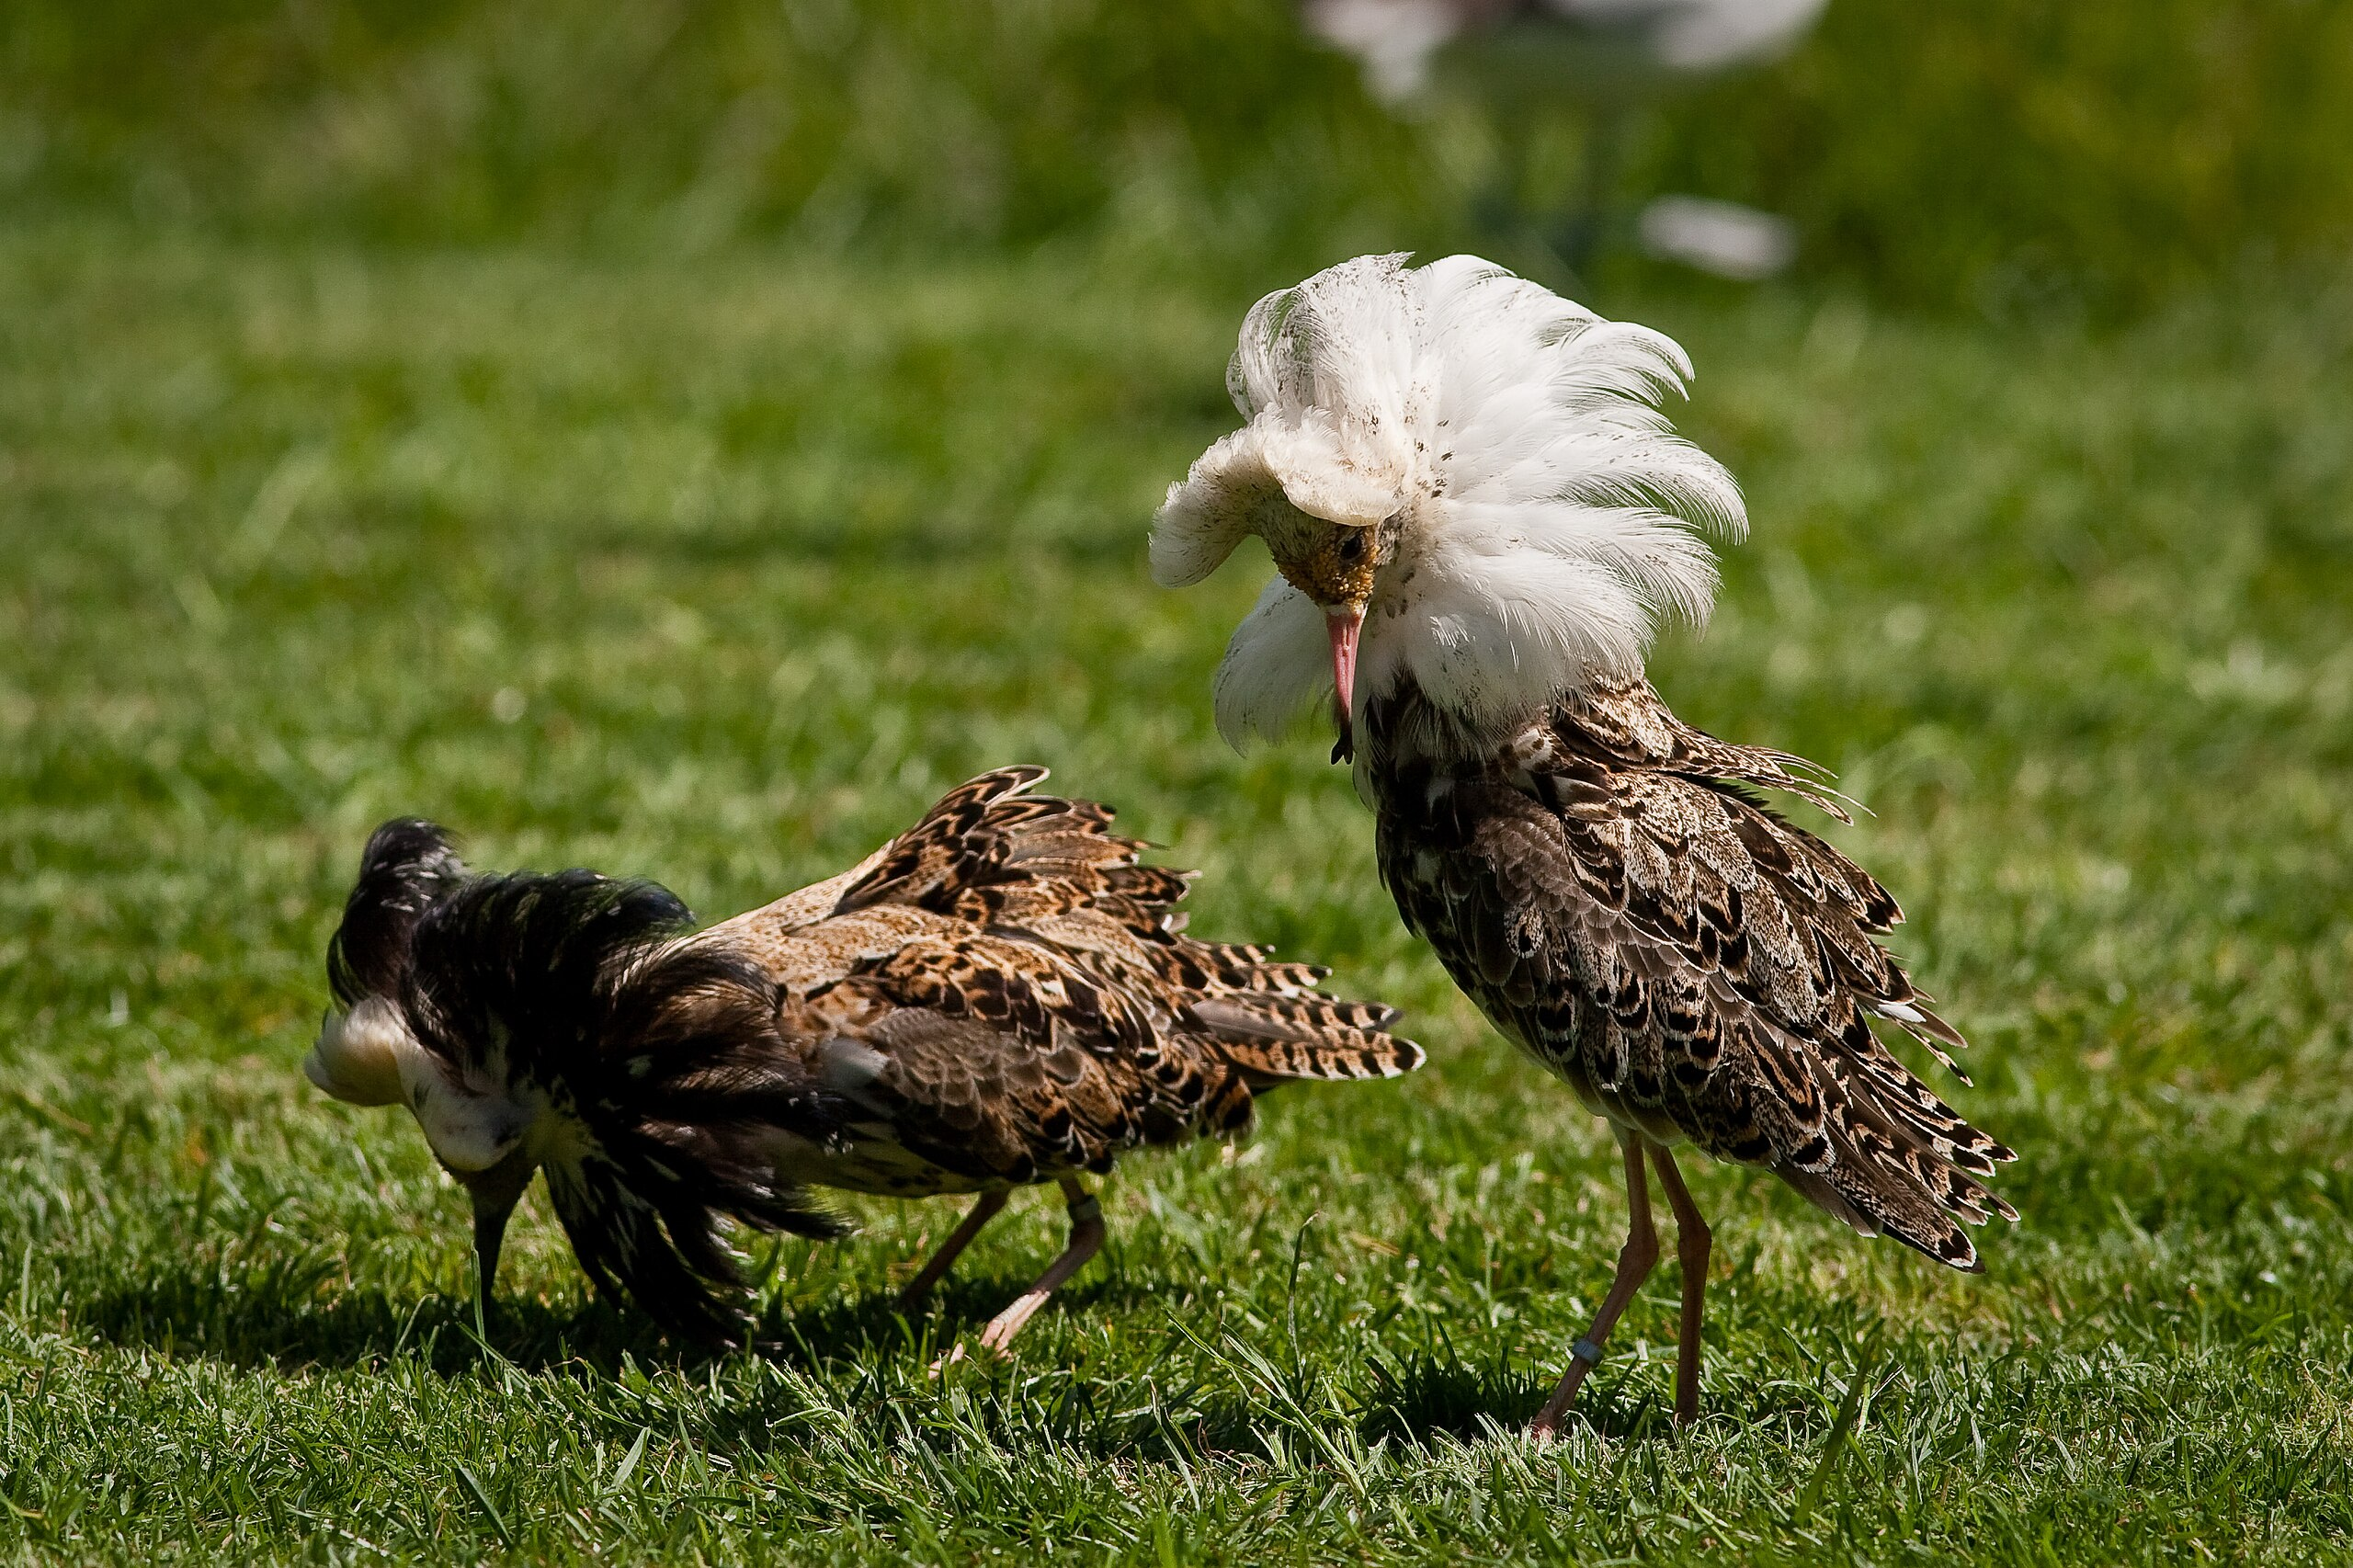
\includegraphics[width=0.8\linewidth, height=3cm, keepaspectratio]{Billeder/Dyr/Fugle/Vadefugle/brushane_han.jpg}\\[0.5em]
        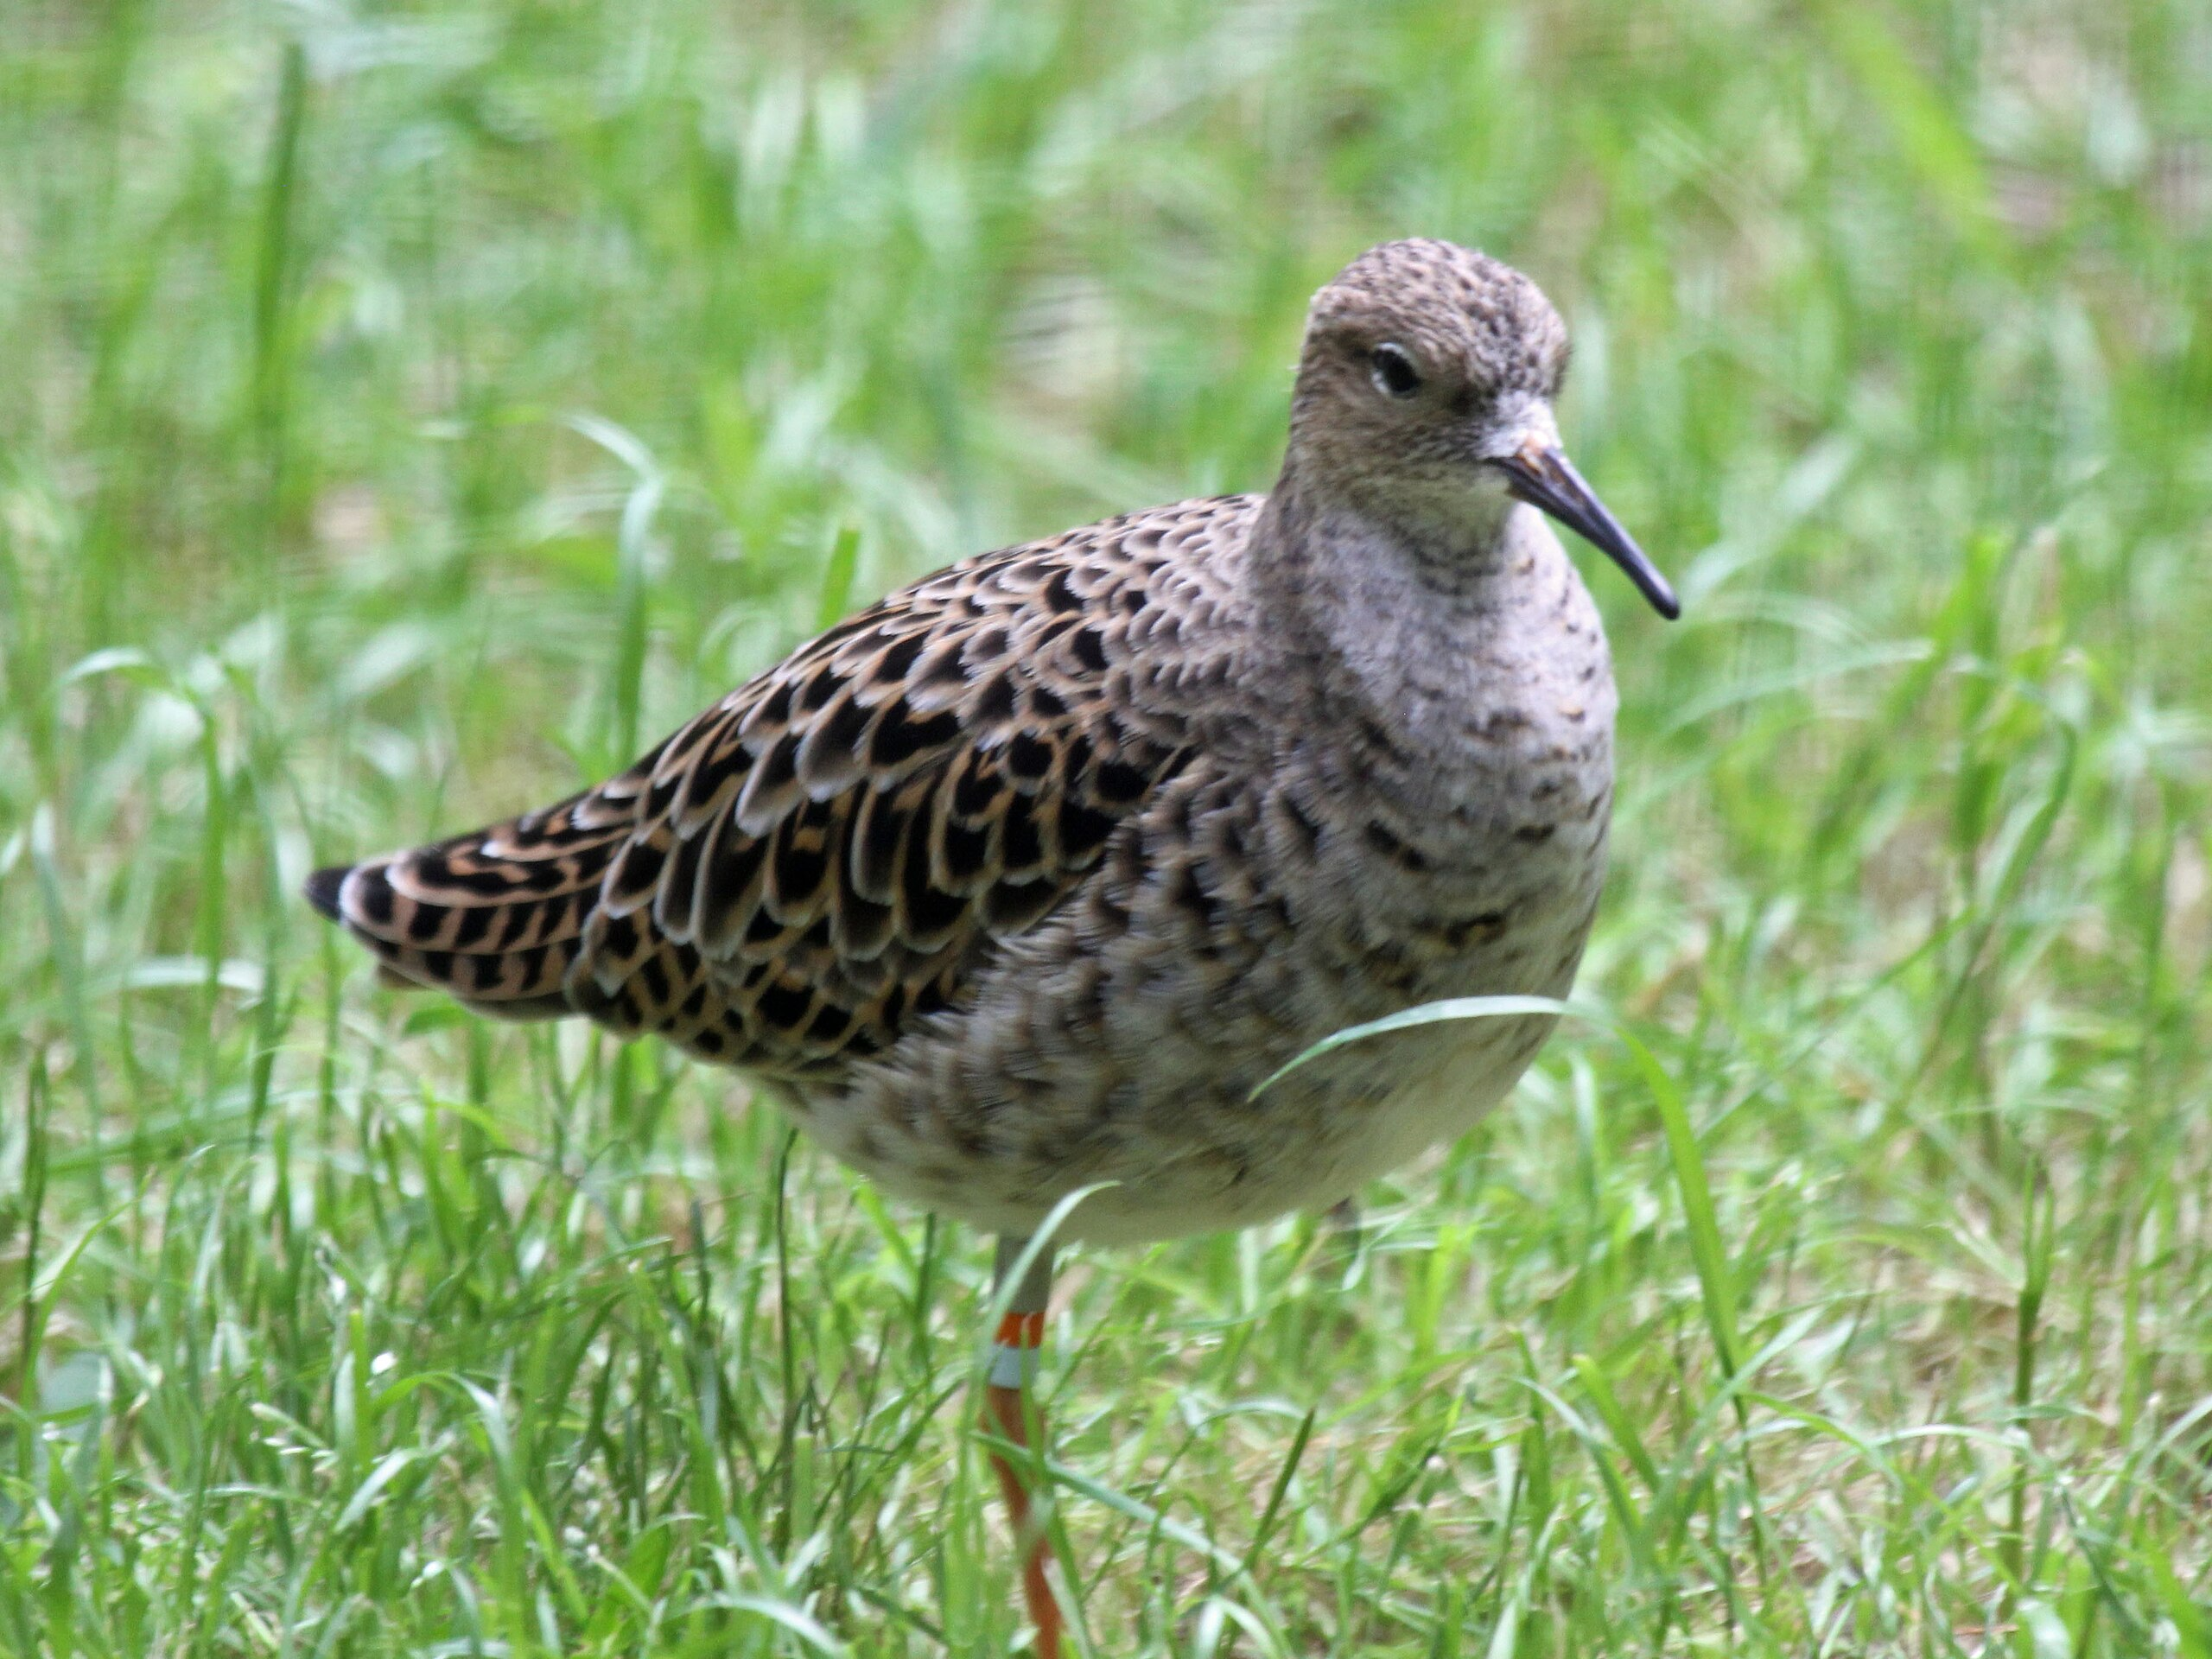
\includegraphics[width=0.8\linewidth, height=3cm, keepaspectratio]{Billeder/Dyr/Fugle/Vadefugle/brushane_hun.jpg}%
      \end{minipage}
    }%
    \vspace{0.05em}
    \footnotesize Han øverst, hun nederst
  \end{columns}
\end{frame}